\documentclass{beamer}
%\usepackage[latin1]{inputenc}
%\usepackage{lmodern}
\usepackage{times}
\usepackage[T1]{fontenc}
\usepackage{graphicx}
\usepackage{bm}
\usepackage{tikz}
\usepackage{verbatim}
\usepackage{amsmath}
\usepackage{booktabs}
\usepackage[small,labelformat=empty]{caption}
\usepackage{url}
\usepackage{colortbl}
\usetikzlibrary{automata,positioning}
\usetikzlibrary{shapes,arrows}

\usetheme{Frankfurt}
%\usetheme{Warsaw}
\title[Title of presentation]{Uhrenbaustein\\
{\small Time&Date and Countdown}
}
\author[author name]
{Tobias F{\"u}lle}
\institute[Fnord GmbH]{Lehrstuhl f{\"u}r integrierte Systeme}
\date{Tue - 06/11/12}


\begin{document}

%{
%\usebackgroundtemplate{\includegraphics[width=\paperwidth]{pictures/sample.jpg}}
%\begin{frame}
%\thispagestyle{empty}
%\titlepage
%\end{frame}
%%}
%%
%\begin{frame}
%\frametitle{Overview}
%\tableofcontents
%\end{frame}
%
%\setlength\fboxsep{5pt}
%\setlength\fboxrule{0pt}

\tikzstyle{state}   = [ rounded rectangle, 
                        draw, 
                        text centered, 
                        minimum height=3em 
                      ]


\section{Time and Date}
%[fragile]
\begin{frame}[fragile]{Time and Date components}
\begin{verbatim} 
component time_date is	
 port(
  current_time:   in  time_signals;
  keyboard_focus: in  std_logic_vector(2 downto 0);
  uni:            in  universal_signals;
  keys:           in  keypad_signals;
  valid:          in  std_logic;
    
  character:     out character_array_2d(3 downto 0,
                                       19 downto 0)
 );
end component;
\end{verbatim}
\end{frame}

\begin{frame}{Time and Date Overview}
  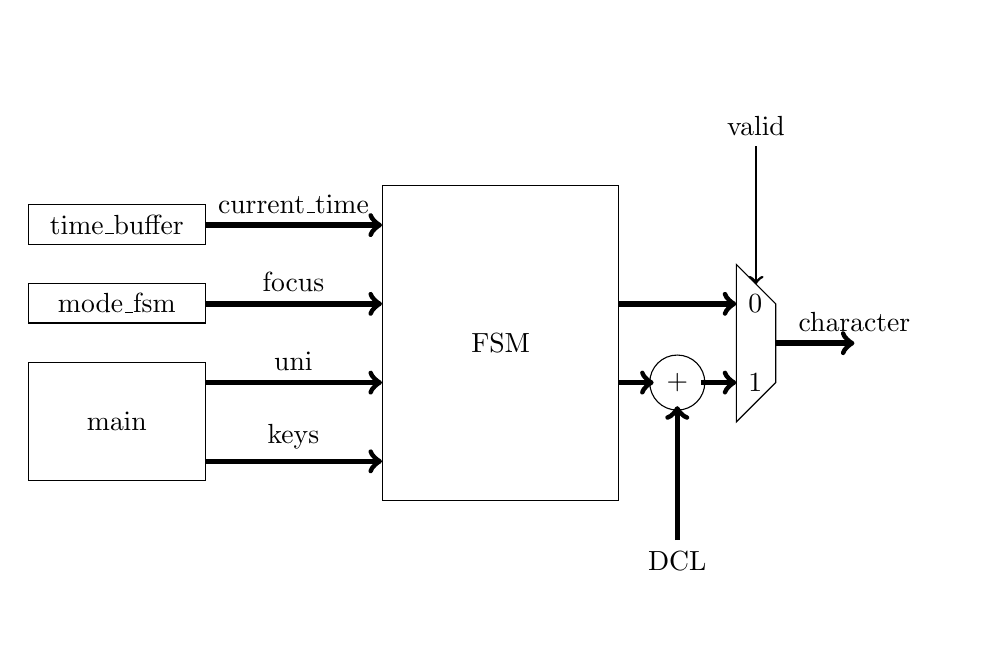
\begin{tikzpicture}
  
\draw[white] (-2.1,.5) rectangle (9, -7);

% individual modules

\node[rectangle,draw=black,minimum height=4cm,minimum width=3cm,above right] at (1.5,-5.5) {FSM};
\node[rectangle,draw=black,minimum height=0.5cm,minimum width=2.25cm,above right] at (-3,-2.25) {time\_buffer};
\node[rectangle,draw=black,minimum height=0.5cm,minimum width=2.25cm,above right] at (-3,-3.25) {mode\_fsm};
\node[rectangle,draw=black,minimum height=1.5cm,minimum width=2.25cm,above right] at (-3,-5.25) {main};
\node[circle,draw=black,inner sep=.12cm] at (5.25, -4) {+};
% mux
\draw (6,-2.5) -- (6.5, -3) -- (6.5,-4) -- (6,-4.5) -- cycle;

% top level module
%\draw[dashed,gray] (-.75,0) rectangle (8.5, -6.25);

% clk/reset signals (enable_gen)
\only<1> {
\draw[line width=2pt,->] (-0.75,-2) -> (1.5, -2) node[midway,above] {current\_time};
\draw[line width=2pt,->] (-0.75,-3) -> (1.5, -3) node[midway,above] {focus};
\draw[line width=2pt,->] (-0.75,-4) -> (1.5, -4) node[midway,above] {uni};
\draw[line width=2pt,->] (-0.75,-5) -> (1.5, -5) node[midway,above] {keys};
\draw[line width=2pt,->] (4.5,-3) -> (6, -3) node[right] {0};
\draw[line width=2pt,->] (5.55,-4) -> (6, -4) node[right] {1};
\draw[line width=2pt,->] (4.5,-4) -> (4.95, -4) ;
\draw[line width=2pt,->] (5.25,-6) node[right, below] {DCL} -> (5.25, -4.3) ;
\draw[line width=1pt,->] (6.25,-1) node[above] {valid} -> (6.25, -2.75) ;
\draw[line width=2pt,->] (6.5,-3.5) -> (7.5, -3.5) node[right, above] {character};
}

\end{tikzpicture}
\end{frame}
\tikzstyle{line}    = [ draw, -latex', text centered, text width = 5cm ]

\begin{frame}{Time and Date FSM}
	\begin{tikzpicture} [text width=1.3cm,align=flush center,font=\normalsize,auto]
		%\node[text width=6cm] at (6,1.2) {All transitions occur on CLK$\uparrow$};
		\node[state] (S0) at (4, -2)  { Display Time };
		\node[state] (S1) at (12, -2) { Display Time \\ and Date };
		
		\path[line] (S0) -- node [right] {mode\_key AND focus} (S1);
		\path[line]	  (S1) -- node {time is up OR reset} (S0);
		\path[line]  (2.5, -0.5) -- (S0);
	\end{tikzpicture}
\end{frame}
  
\begin{frame}[fragile]{Countdown components}
\begin{verbatim} 
component countdown is	
 port(
  keyboard_focus: in  std_logic_vector(2 downto 0);
  uni:            in  universal_signals;
  keys:           in  keypad_signals;
    
  character:     out character_array_2d(3 downto 0,
                                      19 downto 0);
  ti_on:         out std_logic;
  ti_beep:       out std_logic
 );
end component;

\end{verbatim}
\end{frame}  
  
\begin{frame}{Countdown Overview}
  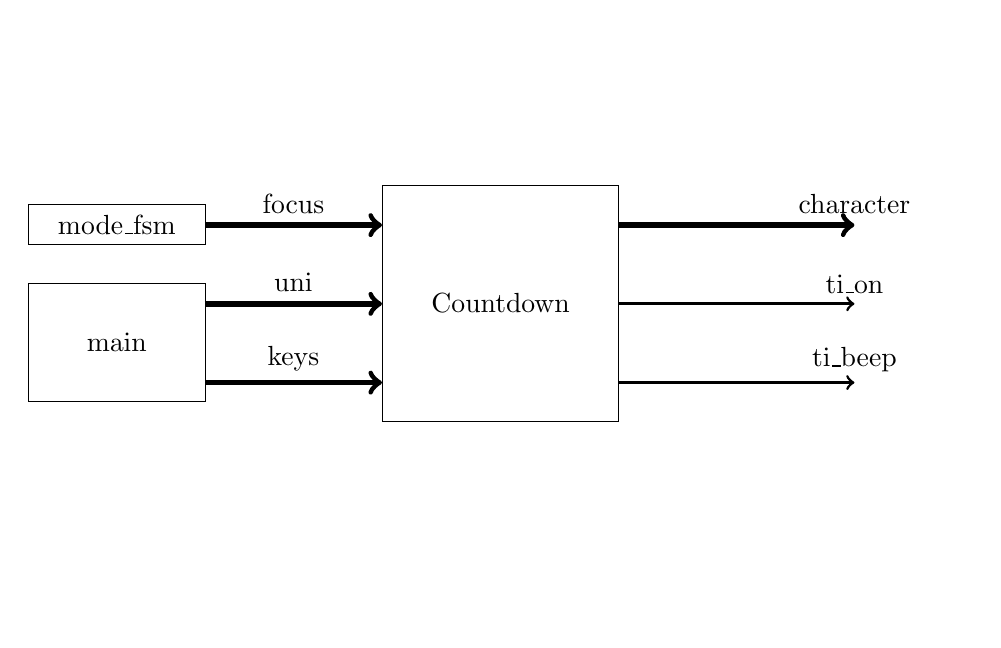
\begin{tikzpicture}
  
\draw[white] (-2.1,.5) rectangle (9, -7);

% individual modules

\node[rectangle,draw=black,minimum height=3cm,minimum width=3cm,above right] at (1.5,-4.5) {Countdown};
\node[rectangle,draw=black,minimum height=0.5cm,minimum width=2.25cm,above right] at (-3,-2.25) {mode\_fsm};
\node[rectangle,draw=black,minimum height=1.5cm,minimum width=2.25cm,above right] at (-3,-4.25) {main};


% clk/reset signals (enable_gen)
\only<1> {
\draw[line width=2pt,->] (-0.75,-2) -> (1.5, -2) node[midway,above] {focus};
\draw[line width=2pt,->] (-0.75,-3) -> (1.5, -3) node[midway,above] {uni};
\draw[line width=2pt,->] (-0.75,-4) -> (1.5, -4) node[midway,above] {keys};
\draw[line width=2pt,->] (4.5,-2) -> (7.5, -2) node[right, above] {character};
\draw[line width=1pt,->] (4.5,-3) -> (7.5, -3) node[right, above] {ti\_on};
\draw[line width=1pt,->] (4.5,-4) -> (7.5, -4) node[right, above] {ti\_beep};
}

\end{tikzpicture}
\end{frame}  
\tikzstyle{line}    = [ draw, -latex', text centered, text width = 2cm ]

\begin{frame}{Time and Date FSM}
	\begin{tikzpicture} [text width=1.3cm,align=flush center,font=\normalsize,auto]
		%\node[text width=6cm] at (6,1.2) {All transitions occur on CLK$\uparrow$};
		\node[state] (S0) at (4, -4.5)  { Set \tiny{\\ti\_on=1\\char=xx:xx}} ;
		\node[state] (S1) at (4, -2) { Reset \tiny{\\time=00:04}};
		\node[state] (S2) at (12, -2) { Start \tiny{\\ti\_on=1\\char=xx:xx}};
		\node[state] (S3) at (12, -4.5) { Beep \tiny{\\ti\_on=0\\ti\_beep=1\\char=xx:xx}};
		\node[state] (S4) at (12, 0.5) { Pause \tiny{\\ti\_on=blink\\char=xx:xx}};
		
		\path[line] (S1) -- (S0);
		\path[line]	  (S0) -- node {Action\_key AND focus} (S2);
		\path[line]  (4, 0) node [centered, above] {reset AND focus} -- (S1);
		\path[line]	  (S2) -- node {Action\_key AND} (S4);
		\path[line]	  (S4) -- node {focus} (S2);
		\path[line]	  (S2) -- node {reaches zero} (S3);
		\path[line]	  (S3) -- (S0);
	\end{tikzpicture}
\end{frame}
  

\end{document}

